% ======================================================================
%  Closed-form collapse loads for a partly embedded pipe (Norwegian)
%  Figure: plots/pipe_formulas.png (plot_pipe_formulas.py)
% ======================================================================
\documentclass[11pt,a4paper]{article}

\usepackage[T1]{fontenc}
\usepackage[utf8]{inputenc}
\usepackage[norsk]{babel}
\usepackage{lmodern}
\usepackage{amsmath,amssymb}
\usepackage{geometry}
\usepackage{graphicx}
\usepackage{booktabs}
\usepackage{caption}
\usepackage{parskip}
\usepackage[hidelinks]{hyperref}

\geometry{left=2.5cm, right=2.5cm, top=2.5cm, bottom=2.5cm}
\graphicspath{{plots/}}
\setlength{\emergencystretch}{3em}

\begin{document}

\begin{center}
  {\LARGE Bruddlast for et delvis nedgravd rør\\[2pt] med skrå overflate}\\[8pt]
  {\large Lukkede formler fra glidelinjefeltet i \texttt{slip-line}}\\[6pt]
  \today
\end{center}

% ----------------------------------------------------------------------
\section{Problemet}
% ----------------------------------------------------------------------

Et stivt rør med radius $R$ ligger i vektløs, udrenert leire (Tresca) med
skjærfasthet $c$.  Det er plan tøyning, og alle krefter er per lengdeenhet
rør.  Røret er trykket ned dybden $P$, målt fra kontaktnivået (der
jordoverflaten møter røret) til rørbunnen.  Kontaktvinkelen, målt ved
rørsenteret fra loddlinja gjennom rørbunnen, er
\begin{equation}
  \varphi = \arccos\Bigl(1 - \frac{P}{R}\Bigr),
  \qquad
  R(1-\cos\varphi) = P,\quad
  R\cos\varphi = R - P,\quad
  R\sin\varphi = \sqrt{P(2R-P)} .
\end{equation}
Grenseflaten har ruhet $r = \tau/c$, der $\tau$ er adhesjonen mellom rør og
jord.  Glidelinjenettet møter røret med vinkelen
\begin{equation}
  \omega = \tfrac12 \arcsin r,
  \qquad
  \sin 2\omega = r,\quad
  \cos 2\omega = \sqrt{1-r^2} .
\end{equation}
Utenfor røret faller overflaten bort fra røret med vinkelen $\theta$; den
er høyest ved røret, og $\theta = 0$ er flat overflate.  Posisjonen langs
kontaktbuen er vinkelen $t$, målt fra rørbunnen.

Figur~\ref{fig:problem} viser de to tilfellene:
\begin{itemize}
  \item \textbf{(a) Sideveis skyv.}  Røret skyves mot høyre.  Bare
        fronthalvdelen ($0 \le t \le \varphi$) har kontakt; jorda bak røret
        løsner.  Skjærspenningen på jorda peker mot frontkanten, så
        friksjonen på røret virker bakover og nedover.  Feltet gir en
        horisontal kraft $H$ og en vertikal kraft $V$.
  \item \textbf{(b) Vertikal nedtrykking.}  Røret trykkes ned, symmetrisk,
        med skråning $\theta$ på begge sider.  Skjærspenningen på jorda
        peker mot rørbunnen, så friksjonen på røret virker oppover.  Feltet
        gir bruddlasten $Q$.
\end{itemize}

\begin{figure}[h]
  \centering
  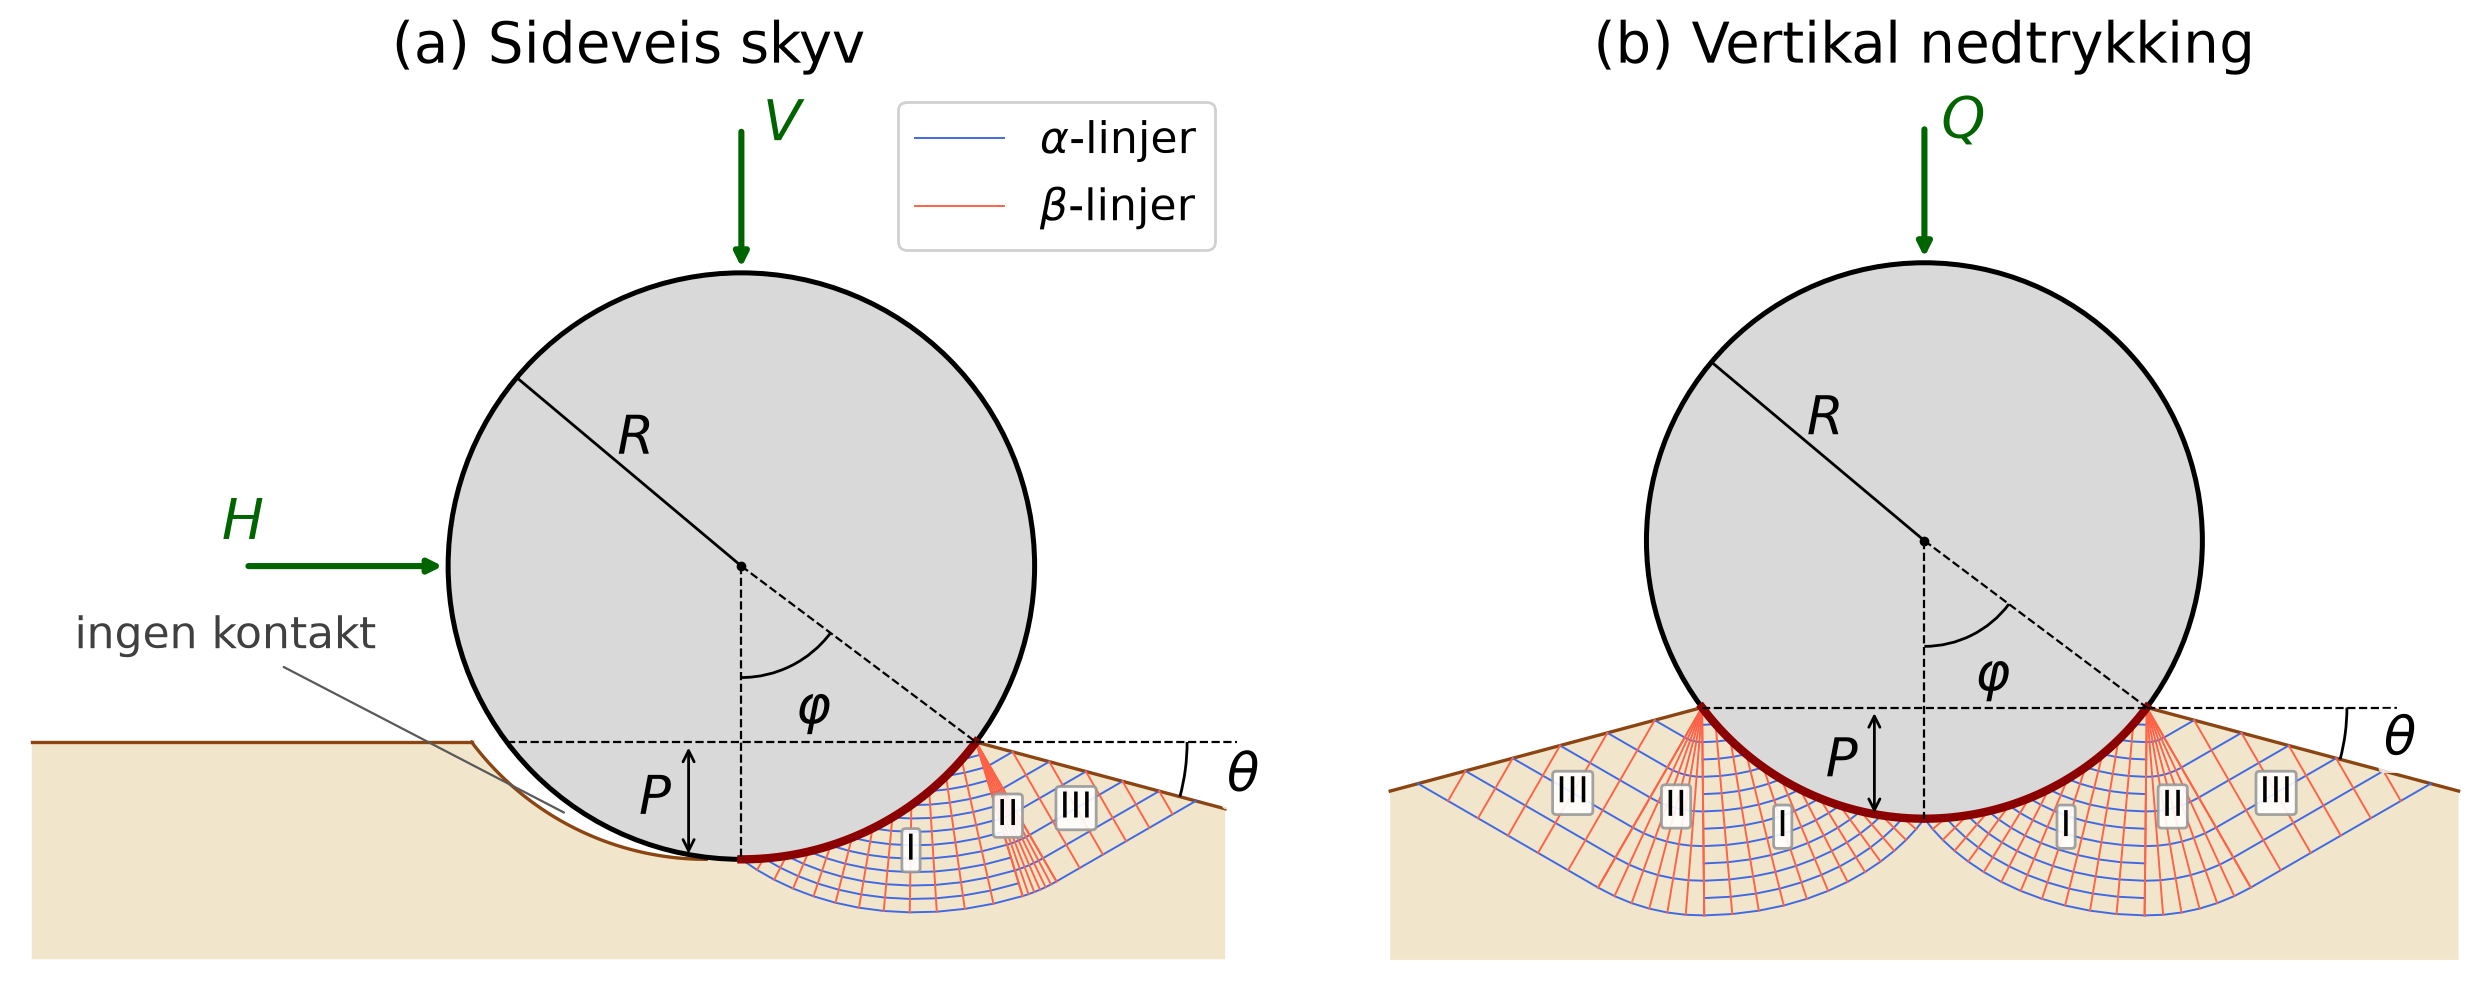
\includegraphics[width=\textwidth]{pipe_formulas.png}
  \caption{De to tilfellene, med glidelinjenettet for $P/R = 0{,}4$,
    $r = 0{,}3$ og $\theta = 15^\circ$.  Kontaktbuen er tegnet med tykk
    rød strek.  I: sonen under røret, II: sentrert vifte i kontaktkanten,
    III: jevn spenningstilstand under den skrå overflaten.  Nettet er det
    fra \texttt{OneSidedDiskSolver} (\texttt{plot\_pipe\_formulas.py}).}
  \label{fig:problem}
\end{figure}

% ----------------------------------------------------------------------
\section{Spenningsfeltet}
% ----------------------------------------------------------------------

Overflaten er fri for spenninger, så i sone~III ligger den største
hovedspenningen $\sigma_1 = 2c$ parallelt med overflaten: middelspenningen
er $\sigma = c$ og hovedspenningsretningen $\psi = \theta$.  I viften
(sone~II) dreier $\psi$ fra $\theta$ til verdien på røret ved kontaktkanten.
På røret er
\begin{equation}
  \psi(t) = \frac{\pi}{2} - t \mp \omega ,
\end{equation}
med øvre fortegn for (a) og nedre for (b).  Langs en $\alpha$-linje fra
overflaten er $\sigma - 2c\psi = c - 2c\theta$, så $\sigma = c(1 + 2\psi -
2\theta)$ på røret.  Mohr-sirkelen gir $\sigma_n = \sigma + c\cos 2\omega$
og $\tau = c\sin 2\omega$, altså
\begin{equation}
  \sigma_n(t) = c\,\bigl(1 + \pi - 2t - 2\theta \mp 2\omega + \cos 2\omega\bigr),
  \qquad
  \tau = r\,c .
  \label{eq:contact}
\end{equation}
Viften åpner seg med vinkelen
\begin{equation}
  \Delta\psi = \frac{\pi}{2} - \varphi \mp \omega - \theta ,
  \label{eq:fan}
\end{equation}
som ikke kan være negativ.  Skråningen senker altså $\sigma_n$ med $2c\theta$
langs hele kontaktbuen, fordi viften blir $\theta$ mindre.  Det er samme
virkning som i $N_c = \pi + 2 - 2\beta$ for et stripefundament på toppen av
en skråning med helning $\beta$.

Kreftene er
\begin{align}
  H &= R\int_0^{\varphi} \bigl(\sigma_n \sin t + \tau\cos t\bigr)\,dt, &
  V &= R\int_0^{\varphi} \bigl(\sigma_n \cos t - \tau\sin t\bigr)\,dt, \\
  Q &= 2R\int_0^{\varphi} \bigl(\sigma_n \cos t + \tau\sin t\bigr)\,dt .
\end{align}
$H$ og $V$ er lastene på røret i (a), mot høyre og nedover.  I (b) gir
begge halvdelene samme bidrag.

% ----------------------------------------------------------------------
\section{Sideveis skyv: $H$ og $V$}
% ----------------------------------------------------------------------

\subsection*{Uten parallellsone, $\varphi \le \pi/2 - \omega - \theta$}

\begin{align}
  \frac{H}{cR} &= \bigl(1 + \pi - 2\omega - 2\theta + \cos 2\omega\bigr)(1-\cos\varphi)
                  + 2\varphi\cos\varphi - (2 - \sin 2\omega)\sin\varphi ,
  \label{eq:H}\\[4pt]
  \frac{V}{cR} &= \bigl(1 + \pi - 2\omega - 2\theta - 2\varphi + \cos 2\omega\bigr)\sin\varphi
                  + (2 - \sin 2\omega)(1-\cos\varphi) .
  \label{eq:V}
\end{align}
Med $P$ og $R$:
\begin{align}
  H &= c\Bigl[\bigl(1 + \pi - 2\omega - 2\theta + \cos 2\omega\bigr)P
        + 2\varphi\,(R-P) - (2 - \sin 2\omega)\sqrt{P(2R-P)}\,\Bigr], \\
  V &= c\Bigl[\bigl(1 + \pi - 2\omega - 2\theta - 2\varphi + \cos 2\omega\bigr)\sqrt{P(2R-P)}
        + (2 - \sin 2\omega)\,P\Bigr].
\end{align}

\subsection*{Med parallellsone, $\pi/2 - \omega - \theta < \varphi \le \pi/2 + \omega - \theta$}

Her ville viften i \eqref{eq:fan} bli negativ.  Som i koden reduseres
ruheten på den ytre buen $t > t_0 = \pi/2 - \omega - \theta$ slik at
$\psi = \theta$ der.  Da er det ingen vifte, og jorda foran den ytre buen er
i samme jevne tilstand som i sone~III ($\sigma_1 = 2c$ langs skråningen).
Den mobiliserte vinkelen er $\omega_\text{eff} = \pi/2 - t - \theta$, og
kontaktspenningen på røret er $2c\sin(t+\theta)\cos\theta$ horisontalt og
$2c\sin(t+\theta)\sin\theta$ vertikalt.  Den indre buen gir
\eqref{eq:H}--\eqref{eq:V} med $\varphi = t_0$:
\begin{align}
  \frac{H}{cR} &= \underbrace{(1+\cos 2\omega)\bigl(1-\sin(\omega+\theta)\bigr)
                  + (\sin 2\omega - 2)\cos(\omega+\theta) + \pi - 2\omega - 2\theta}_{\text{indre bue, } 0 \le t \le t_0} \nonumber\\
               &\quad + \underbrace{2\cos\theta\,\bigl(\sin\omega - \cos(\varphi+\theta)\bigr)}_{\text{ytre bue, } t_0 < t \le \varphi} \nonumber\\
               &= 1 + \pi - 2\omega - 2\theta + \cos 2\omega
                  + 2(\sin\omega - \cos\omega)(\sin\theta + \cos\theta)
                  - 2\cos\theta\cos(\varphi+\theta) ,
  \label{eq:Hpar}\\[6pt]
  \frac{V}{cR} &= \underbrace{(1+\cos 2\omega)\cos(\omega+\theta)
                  + (2 - \sin 2\omega)\bigl(1-\sin(\omega+\theta)\bigr)}_{\text{indre bue}}
                 \;+\; \underbrace{2\sin\theta\,\bigl(\sin\omega - \cos(\varphi+\theta)\bigr)}_{\text{ytre bue}} \nonumber\\
               &= 2 - \sin 2\omega + 2(\cos\omega - \sin\omega)(\cos\theta - \sin\theta)
                  - 2\sin\theta\cos(\varphi+\theta) .
  \label{eq:Vpar}
\end{align}
De to tilfellene gir samme verdi ved $\varphi = \pi/2 - \omega - \theta$.
Med $\theta = 0$ blir det ytre bidraget til $V$ null, fordi $\sigma_1$ da
er horisontal.

\subsection*{Gyldighet}

Formlene gjelder for $\varphi \le \pi/2 + \omega - \theta$.  For større
$\varphi$ måtte den ytre buen ha $\omega_\text{eff} < -\omega$, altså skjær
i motsatt retning som er større enn $rc$.  For glatt rør betyr det
$P/R \le 1 - \sin\theta$ (0,74 ved $\theta = 15^\circ$, 0,50 ved
$\theta = 30^\circ$), og bare \eqref{eq:H}--\eqref{eq:V} er i bruk.  For ru
rør gjelder formlene alltid når $\theta \le \omega$, ellers for
$P/R \le 1 - \sin(\theta - \omega)$.

% ----------------------------------------------------------------------
\section{Vertikal nedtrykking: $Q$}
% ----------------------------------------------------------------------

\begin{align}
  \frac{Q}{cR} &= 2\Bigl[\bigl(1 + \pi + 2\omega - 2\theta - 2\varphi + \cos 2\omega\bigr)\sin\varphi
                  + (2 + \sin 2\omega)(1-\cos\varphi)\Bigr], \\
  Q &= 2c\Bigl[\bigl(1 + \pi + 2\omega - 2\theta - 2\varphi + \cos 2\omega\bigr)\sqrt{P(2R-P)}
        + (2 + \sin 2\omega)\,P\Bigr].
\end{align}
Formelen gjelder for $\varphi \le \pi/2 + \omega - \theta$, der viften
\eqref{eq:fan} ikke er negativ.  Her finnes det ingen parallellsone: den
ville kreve mer enn full ruhet (koden gir feilmelding).  For glatt rør er
grensen den samme som i (a), $P/R \le 1 - \sin\theta$.

Kontroll: med $\theta = 0$ og $r = 0$ gir $P = R$ bruddlasten $Q = 8cR = 4cD$,
og $P/R = 0{,}5$ gir $Q/(cD) = 3{,}639$, som i manualen.

% ----------------------------------------------------------------------
\section{Merknader}
% ----------------------------------------------------------------------

\begin{itemize}
  \item \textbf{Kombinert last.}  I (a) hører $H$ og $V$ sammen: feltet
        beskriver brudd under lastkombinasjonen $(V, H)$.  Det er ikke
        bæreevnen for ren horisontal last ($V = 0$), og heller ikke den
        største $H$ for en gitt $V$.
  \item \textbf{Ruhet.}  Formlene forutsetter full friksjon, $|\tau| = rc$,
        langs hele buen (unntatt parallellsonen).  En grenseflate med ruhet
        $r$ kan alltid mobilisere mindre, så feltene for alle $r' \le r$ gir
        lastkombinasjoner $(V, H)$ som et ru rør også kan bære.  Det betyr
        noe fordi $H$ ikke alltid øker med $r$: ved $P/R = 0{,}5$ og
        $\theta = 0$ er $H/(cR) = 1{,}990$ for $r = 0{,}5$, men $1{,}571$ for
        $r = 1$ (tabell~\ref{tab:values}).
  \item \textbf{Ikke bevist nedre grense.}  Spenningsfeltet dekker bare de
        plastiske sonene og er ikke vist å kunne utvides inn i den stive
        jorda.  For det flate vertikale tilfellet gjør hastighetsfeltet på
        det samme nettet negativt plastisk arbeid i deler av sonen, så det
        er heller ikke en komplett løsning.  Den øvre-grense-mekanismen i
        \texttt{PipeLateral} bærer noen prosent mindre vertikal last for et
        ru rør enn spenningsløsningen.
  \item \textbf{Rett skråning.}  Overflaten er en rett linje fra
        kontaktkanten.  \texttt{PipeLateral} tilpasser en rett linje til
        bermen på samme måte.
\end{itemize}

% ----------------------------------------------------------------------
\section{Kontroll mot koden}
% ----------------------------------------------------------------------

Formlene er sammenlignet med numerisk integrasjon av kontaktspenningene i
koden:
\begin{itemize}
  \item \texttt{OneSidedDiskSolver} med \texttt{phi\_start=0},
        \texttt{omega} $= \pm\omega$ og \texttt{alpha} $= \theta$;
  \item for $\theta = 0$ også \texttt{forces\_on\_half\_disk()} og
        \texttt{collapse\_load\_Q()} i \texttt{DiskPrandtlSolver}
        (den siste med \texttt{vertical\_shear=True}).
\end{itemize}
Avviket er under $10^{-8}\,cR$ for $P/R = 0{,}02$--$1$, $r = 0$--$1$ og
$\theta = 0$--$30^\circ$ innenfor gyldighetsområdet.

Sammenhengen med koden:
\begin{itemize}
  \item $P = pD$, der \texttt{p} er nedtrykkingsforholdet i
        \texttt{DiskFoundationBoundary};
  \item $\varphi$ er \texttt{theta\_max}, og $\theta$ er \texttt{alpha} i
        \texttt{OneSidedDiskSolver};
  \item $+\omega$ gjelder (a), som er standardretningen, og $-\omega$
        gjelder (b), med \texttt{vertical\_shear=True}.
\end{itemize}

\begin{table}[h]
  \centering
  \caption{Kontrollverdier.  $^*$: med parallellsone i (a).
    --: utenfor gyldighetsområdet.}
  \label{tab:values}
  \begin{tabular}{ccc ccc}
    \toprule
    $P/R$ & $r$ & $\theta$ & $H/(cR)$ & $V/(cR)$ & $Q/(cR)$ \\
    \midrule
    0{,}2 & 0{,}0 & $0^\circ$ & 0{,}858 & 2{,}713 & 5{,}426 \\
    0{,}2 & 0{,}5 & $0^\circ$ & 1{,}026 & 2{,}218 & 6{,}093 \\
    0{,}2 & 1{,}0 & $0^\circ$ & 0{,}944 & 0{,}970 & 6{,}510 \\
    0{,}5 & 0{,}0 & $0^\circ$ & 1{,}886 & 3{,}639 & 7{,}278 \\
    0{,}5 & 0{,}5 & $0^\circ$ & 1{,}990 & 2{,}819 & 8{,}453 \\
    0{,}5 & 1{,}0 & $0^\circ$ & 1{,}571$^*$ & 1{,}000 & 9{,}267 \\
    1{,}0 & 0{,}0 & $0^\circ$ & 3{,}142 & 4{,}000 & 8{,}000 \\
    1{,}0 & 0{,}5 & $0^\circ$ & 3{,}070$^*$ & 2{,}914 & 9{,}779 \\
    1{,}0 & 1{,}0 & $0^\circ$ & 2{,}571$^*$ & 1{,}000 & 11{,}142 \\
    \midrule
    0{,}2 & 0{,}0 & $15^\circ$ & 0{,}753 & 2{,}399 & 4{,}797 \\
    0{,}2 & 0{,}5 & $15^\circ$ & 0{,}922 & 1{,}904 & 5{,}465 \\
    0{,}2 & 1{,}0 & $15^\circ$ & 0{,}854$^*$ & 0{,}680 & 5{,}882 \\
    0{,}5 & 0{,}0 & $15^\circ$ & 1{,}624 & 3{,}186 & 6{,}371 \\
    0{,}5 & 0{,}5 & $15^\circ$ & 1{,}728 & 2{,}366 & 7{,}546 \\
    0{,}5 & 1{,}0 & $15^\circ$ & 1{,}547$^*$ & 0{,}866 & 8{,}360 \\
    1{,}0 & 0{,}0 & $15^\circ$ & -- & -- & -- \\
    1{,}0 & 0{,}5 & $15^\circ$ & 2{,}728$^*$ & 2{,}634 & 8{,}732 \\
    1{,}0 & 1{,}0 & $15^\circ$ & 2{,}547$^*$ & 1{,}134 & 10{,}094 \\
    \bottomrule
  \end{tabular}
\end{table}

\end{document}
